\documentclass{article}
\title{Atomic Force Microscopy of Titin}
\author{Zachariah Sachs (with Jeff Montgomery)}
\usepackage{graphicx}
\usepackage{float}

\begin{document}
\maketitle
\section{Purpose}

In this laboratory exercise, we took many measurements of one type of
single-molecule pulling event in order to explore the worm-like chain (WLC)
model of polymer mechanics and the principles of cantilever-force microscopy via statistical
analysis from several viewpoints.

\section{Theory and Methods}

Atomic force microscopy (AFM) informs upon interatomic force potentials 
between the tip of a cantilever and an image substance at atomic distances.
Three-dimensional displacement-force data collected by rastering the tip accross a surface
allows for imaging topography. One dimensional displacement-force data collected by 
bouncing the tip in a solution of polymers allows for the investigation of the mechanics
of polymer folding.

The movement and deflection of an AFM cantilever is detected optically and controlled
electronically. A laser reflected off the back of the cantilever,
necessarily made of material with an appropriate refractive index, impinges on a
position-sensitive detector, usually a photodiode, to track the deflection of the cantilever.
Feedback electronics sensitive to potential differences at the detector keep the cantilever
under control and prevent it from vibrating. Electronically sensitive materials, 
piezoelectric transducers, react to differences in applied potentials, either from a feedback
loop or a control signal, to control the displacement of the cantilever. These elements are
assembled into a digital circuit and controlled by a computer.

Treating the cantilever as an ideal spring, the deflection mechanics can be modeled by
Hooke's Law and extracted from its geometry and material via Young's modulus
\footnote{See procedure, equations (1) through (6)}. The
Young's modulus also determines the natural resonance frequency of the spring. The
software used to control the tip requires the spring constant of this ideal spring to
callibrate measurements of force deflection and to damp the vibrations through feedback.

The worm-like chain (WLC) model treats polymers as smoothly curved flexible rods.
The rod ``remembers'' its direction at an initial point to a distance $s$ along the curve
according to $e^{-s/P}$ where $P$ is the persistence length of the chain. This decay
is a result of thermal energy and the persistence length indicates stiffness of the fiber.
For $L_C$ the end-to-end distance of the fully extended polymer segment, called the
contour length, and $P$ the persistence length, the WLC model gives the force $F$ needed
to extend the polymer a distance $x$ as
\begin{equation}
F_{WLC}(x,P,L_C)=\frac{k_B T}{P} \left(\frac{1}{4}
\left(1-\frac{x}{L_C}\right)^{-2}-\frac{1}{4}
+\frac{x}{L_C}\right).
\end{equation}

Titin in a a mammalian muscle fiber protein consisting of 34,350 amino acids that spans
about 1 $\mu$m and contains approximately 300 immunoglobulin (Ig) domains. This gives
an estimate of 29 pm for the length of an amino acid backbone. I270 titin is
a recombinant form from cardiac muscle which contains repeats of one specific Ig domain.

We used a Bioscope AFM system with the Nanoscope IIIa Controller from Digital Instruments
to analyze I270 titin \footnote{AthenaES, AES 0304-C100, Baltimore MD} which is
engineered to consist of eight Ig27 domain repeats. The protein was bound to a gold coated 
and annealed mica substrate on a microscope slide \footnote{Agilent Technologies, Santa 
Clara CA}. A BioLever BL-RC-150 VB \footnote{Asylum Research, Inc.} of type 2A with
Hooke's Law spring constant approximately $0.03 N/m$ made of silicon nitride and
coated with chromium and gold was used. First, the resonant frequency of the cantilever
was tuned in air using the computer software. The protein sample and cantilever were
then placed in the AFM assembly and immersed together in a solution of phosphate saline
buffer (PBS). The cantilever was retuned in PBS. The software bounced the cantilever,
pressing it into the slide enough to displace the tip, and then retracted, with the intention
that the tip would bind to one part of a titin fiber that was stuck to the slide and would
stretch it out. The extension-retraction data was visualized on the computer and force data
which demonstrated the saw-tooth shape characteristic of the sequential stressing and
unfolding of the Ig domains were stored to the computer.

The first cantilever we used broke between tuning it in air and in PBS. Replacement took
some time, and our titin slide dried out for a few minutes. We rewetted it with
PBS and hoped for the best. In the interest of time, we were not terribly picky about the laser
tuning parameters. Given these delays, we were only able to collect sixteen good
force-extension curves.

\section{Data and Plots}

\subsection{Temperature}

We neglected to take the temperature the day of. Given that the laboratory is in a climate
controlled building, I estimate the air temperature to within 10 degrees of $72^\circ F$.

\subsection{Force Extension Curves and Histograms}

A representative protein force-extension curve printed by
MATLAB\footnote{MATLAB script \texttt{zs\textunderscore raw.m}.} from collected data is
provided in Figure 1.
The cantilever tip is first forced into the sample slide generating the peak/plateau
on the left of the plot below. Positive force here pushes the tip up. As the tip is retracted,
attached titin molecules pull on the tip, giving a negative force, and are themselves
extended by the equal and opposite force.
When an Ig domain ruptures, the tip relaxes towards equilibrium, generating a
``peak''---a local force minimum.
The AFM was subject to mechanical vibrations that were large relative to the atomic
measurement distances and tip deflections, so it was impossible to calibrate an absolute
force zero. In the analysis, the relatively constant section of the curve to the right of the
last force peak is used to calibrate the data to zero. We expect eight Ig domain rupture
peaks for I270 titin.

\begin{figure}[H]
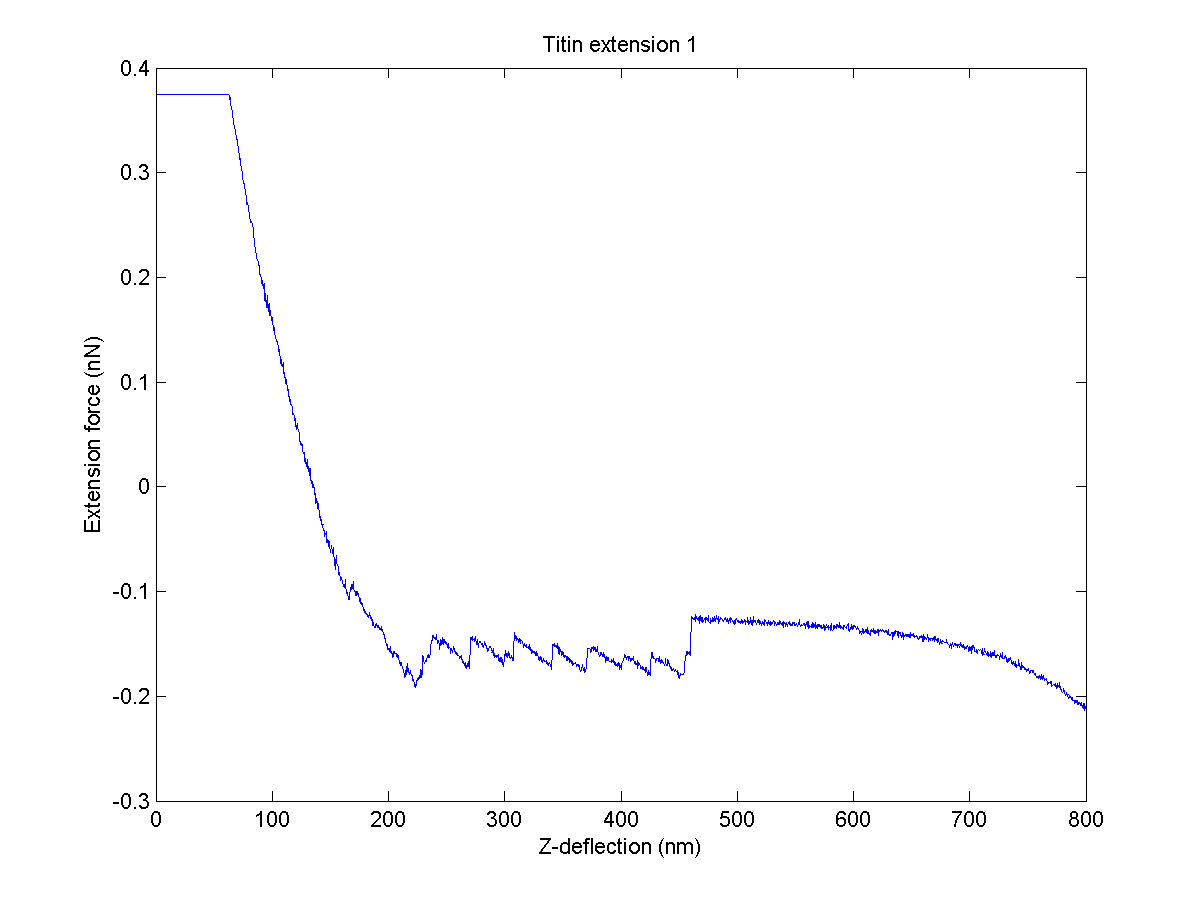
\includegraphics[width=0.8\textwidth]{dd1}
\centering
\caption{Representative protein force-extension curve.}
\end{figure}

We can also visualize this data as a histogram. The plateau from the force-extension curve
appears as a large bar to the far right. A distribution corresponding to the rupture peaks 
appears around -0.2 nN. Large bars corresponding to the fairly constant section at the
end appear just above that.

\begin{figure}[H]
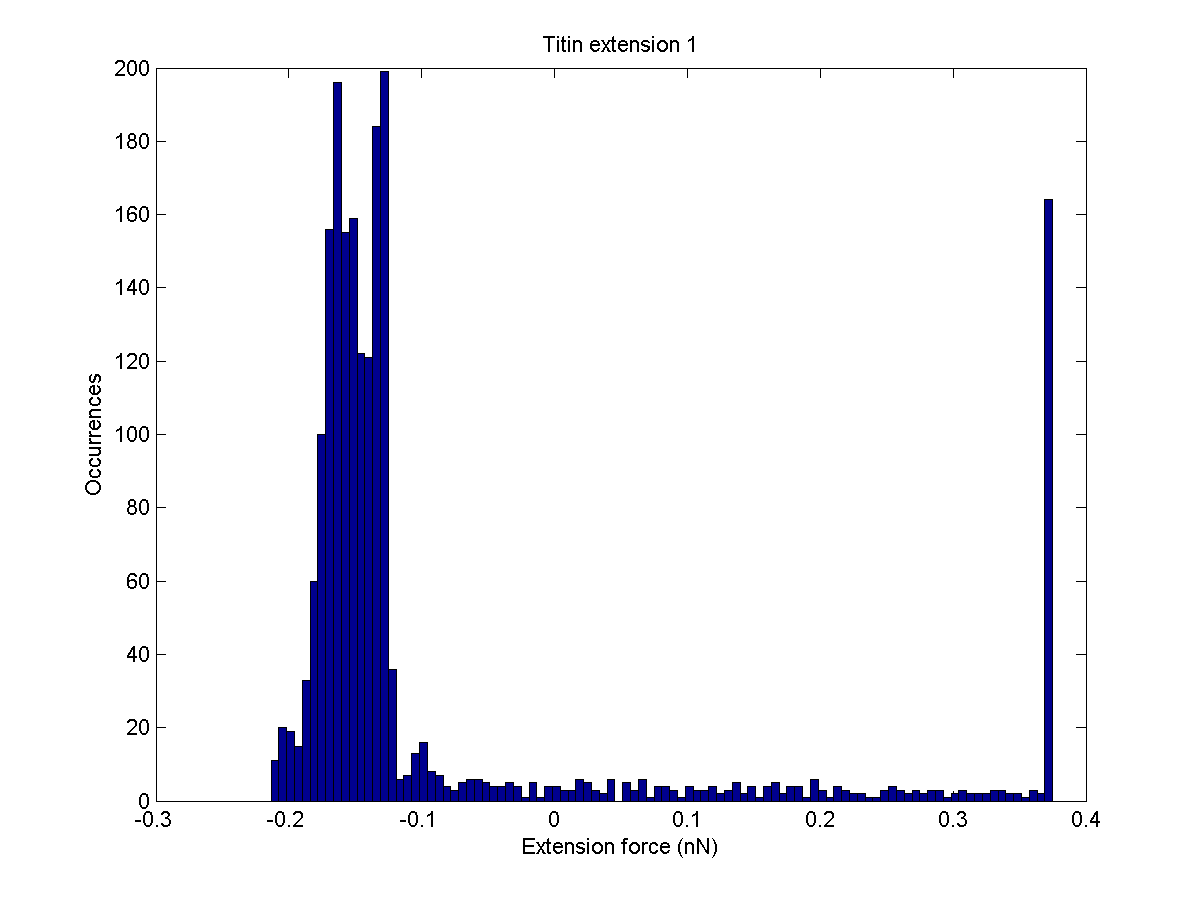
\includegraphics[width=0.8\textwidth]{hh1}
\centering
\caption{Representative histogram of protein extension forces from Figure 1 showing a
distribution of rupture peak forces arround -0.2 nN.}
\end{figure}

\section{Analysis}

\subsection{Data Manipulation}

First, I inverted the force data to correspond to the positive force applied by titin to the
AFM cantilever.
Using included MATLAB analysis functions\footnote{MATLAB function 
\texttt{[pks,locs]=findpeak(data,'Name',value)} in scripts \texttt{zs\textunderscore 
ptp\textunderscore fl.m} and \texttt{zs\textunderscore rupture.m}.},
I then visually analysed the inverted force extension curves to mark the Ig domain
rupture events. Ideally, data collected after the last rupture event corresponds to zero
applied force. So, we might zero the force scale to the average of the post-rupture
data\footnote{MATLAB script \texttt{zs\textunderscore rupture.m}.}. 
However, Figure 1 shows that this data is hardly constant, and even varies on a scale larger
than the rupture force peaks. I cannot specifically justify excluding some of this
post-rupture data, so I continue with the uncertainty introduced by this manipulation.
An example of inverted and zeroed force-extension data with Ig domain rupture events
marked is included in Figure 3.

\begin{figure}[H]
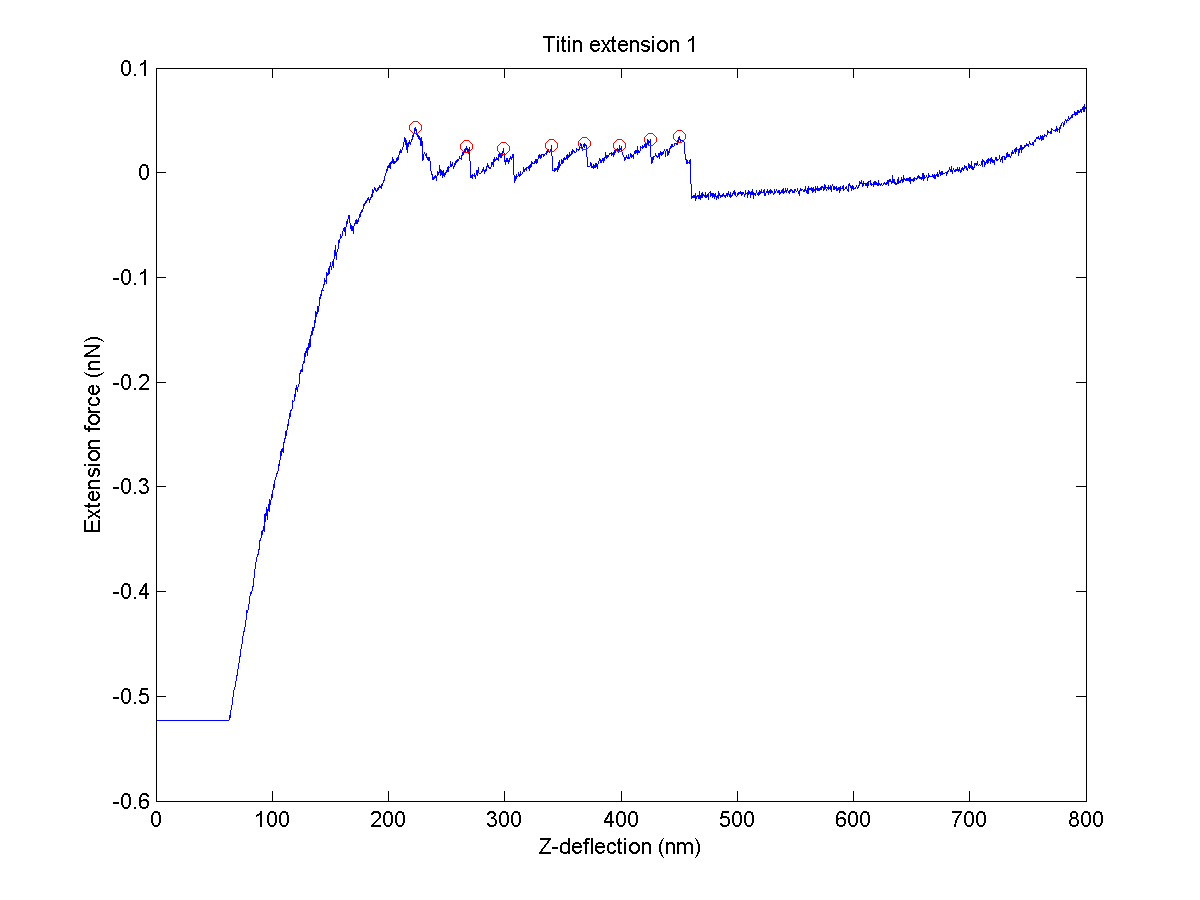
\includegraphics[width=0.8\textwidth]{psh1}
\centering
\caption{Inverted and force-zeroed protein force-extension curve showing eight Ig
domain rupture events.}
\end{figure}

\subsection{Domain Contour Length: Average Over Force Peaks}

The tip-displacement between the first and last marked Ig domain rupture events divided
by the number of marked rupture events for each force-extension curve is plotted below in
Figure 4 and fit with a Gaussian
distribution\footnote{MATLAB script \texttt{zs\textunderscore ptp\textunderscore fl.m}.}.
These values give a rough average of the
contour length $L_c$ of an individual extended Ig domain as the extended length of the 
stretched protein over the number of intermediate folding domains. The Gaussian fit gives
the contour length as 26.7 nm with a standard of deviation 7.0 nm.

\begin{figure}[H]
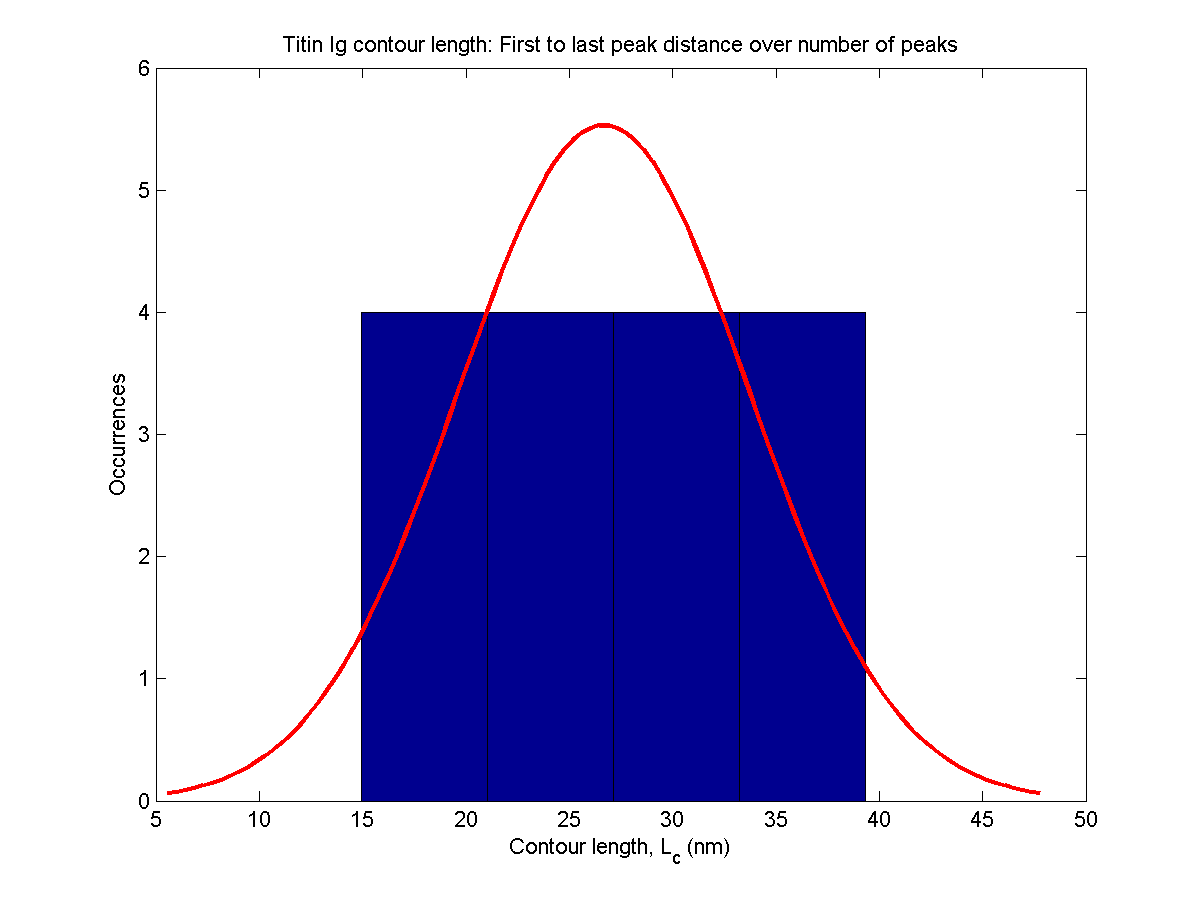
\includegraphics[width=0.8\textwidth]{hisfl}
\centering
\caption{Ig domain first to last rupture event displacement over number of events for each
molecular pulling measurement fitted with a Gaussian distribution.}
\end{figure}

There are a number of reasons why we should expect a nonzero variance for this value.
Nanomeasurement are subject to mechanical uncertainty. Manufacturing
instruments as small as the cantilever to within 10\% of given specifications is impressive.
Isolating such tiny components from much larger mechanical vibrations is also a challenge.
The technique of the single-molecule pulling measurement, in which the delicate cantilever 
was bounced vigorously (as demonstrated by the initial plateau in Figure 1), limits the 
absolute calibration of zero. 
Statistical uncertainties due to thermal noise are inherent to measurements involving 
electronics.  Further, controls in  software and circuitry used to 
compensate for mechanical uncertainty are subject to a time delay. For example,  the
feedback loops that prevent the cantilever from resonating must respond to optical
detection by piezoelectric transducers.
The randomness of single-molecule pulling events contributes uncertainty as well. We
cannot be sure which chunks of polymer stick to the probe and to the slide, so we don't 
know which Ig domains we are analysing. The polymer may only be bound so well to the
slide surface, so it might break lose in the middle of an Ig domain stretch. Though we try
to control the environment, the polymer may be in any random state of folding. As we stretch 
the polymer, the number of folded domains available changes, introducing randomness
through combinatorics. We treat
the deflection of the cantilever as a one dimensional problem, ignoring other dimensions of
pulling and torsion. Random mutations of the peptide sequence also contribute. 

\subsection{Domain Contuor Length: Peak-to-Peak Distribution}

The tip-displacement between marked Ig domain rupture events is plotted below in
Figure 5 and fit with a Gaussian
distribution\footnote{MATLAB script \texttt{zs\textunderscore ptp\textunderscore fl.m}.}.
These values correspond to the contour length $L_c$ of a specific extended Ig domain.
The Gaussian fit gives the contour length as 30.6 nm with a standard of 
deviation 14.7 nm.

\begin{figure}[H]
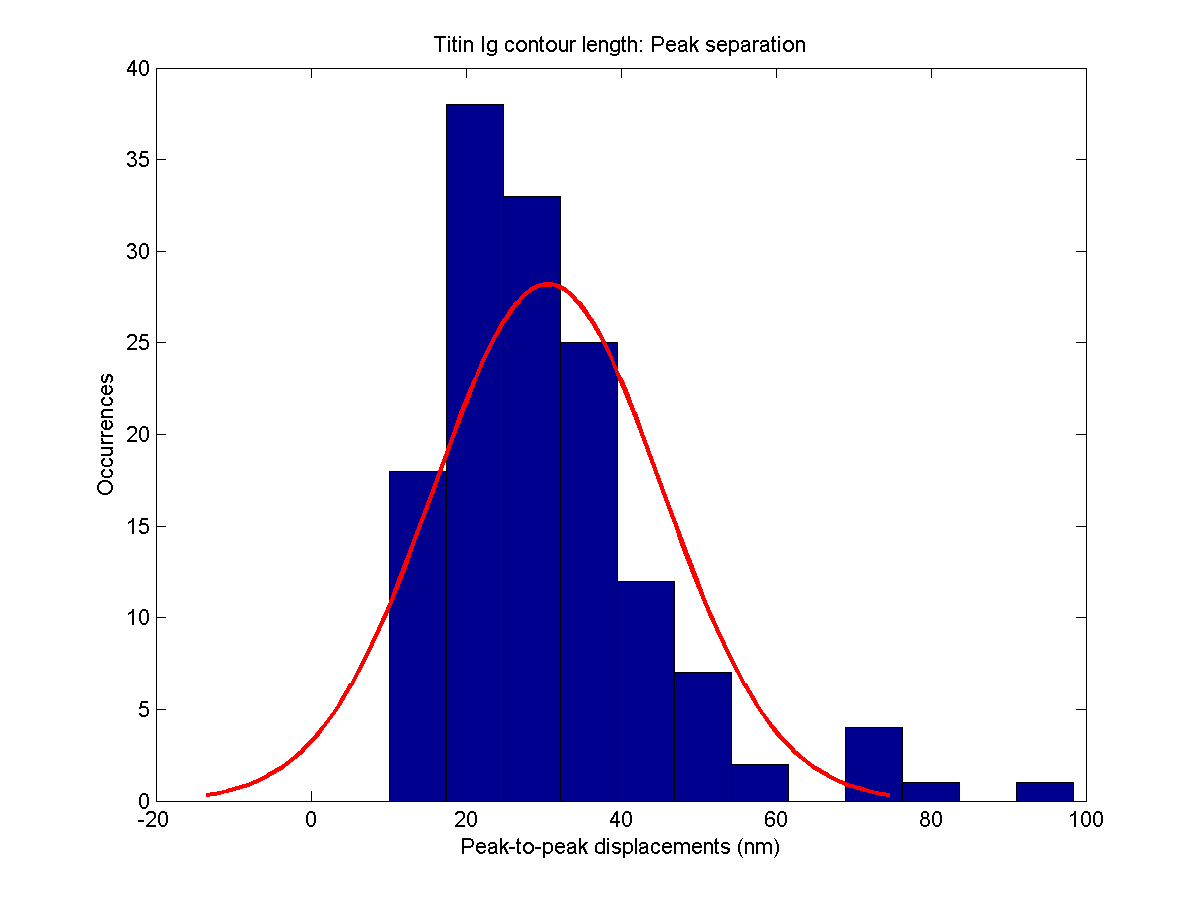
\includegraphics[width=0.8\textwidth]{hisptp}
\centering
\caption{Ig domain rupture peak-to-peak displacement fitted with a 
Gaussian distribution.}
\end{figure}

This value of $L_c$ is subject to the same uncertainties as the first to last over peaks
value. I want to reemphasize here the contribution of random folding, combinatorics,
and random mutations, since here we are taking the average of individual displacements,
not, as above, the average of an average of displacemens. Notice how this histogram is not as smooth as that above, and shows more outliers.

\subsection{Domain Rupture Force}

The Ig domain rupture force, zeroed and marked as discussed above, is plotted below in
Figure 6 and fitted with a Gaussian 
distribution\footnote{MATLAB script \texttt{zs\textunderscore rupture.m}.}.
The Gaussian fit gives the rupture force as 44.0 pN with a standard of deviation
24.6 pN.

\begin{figure}[H]
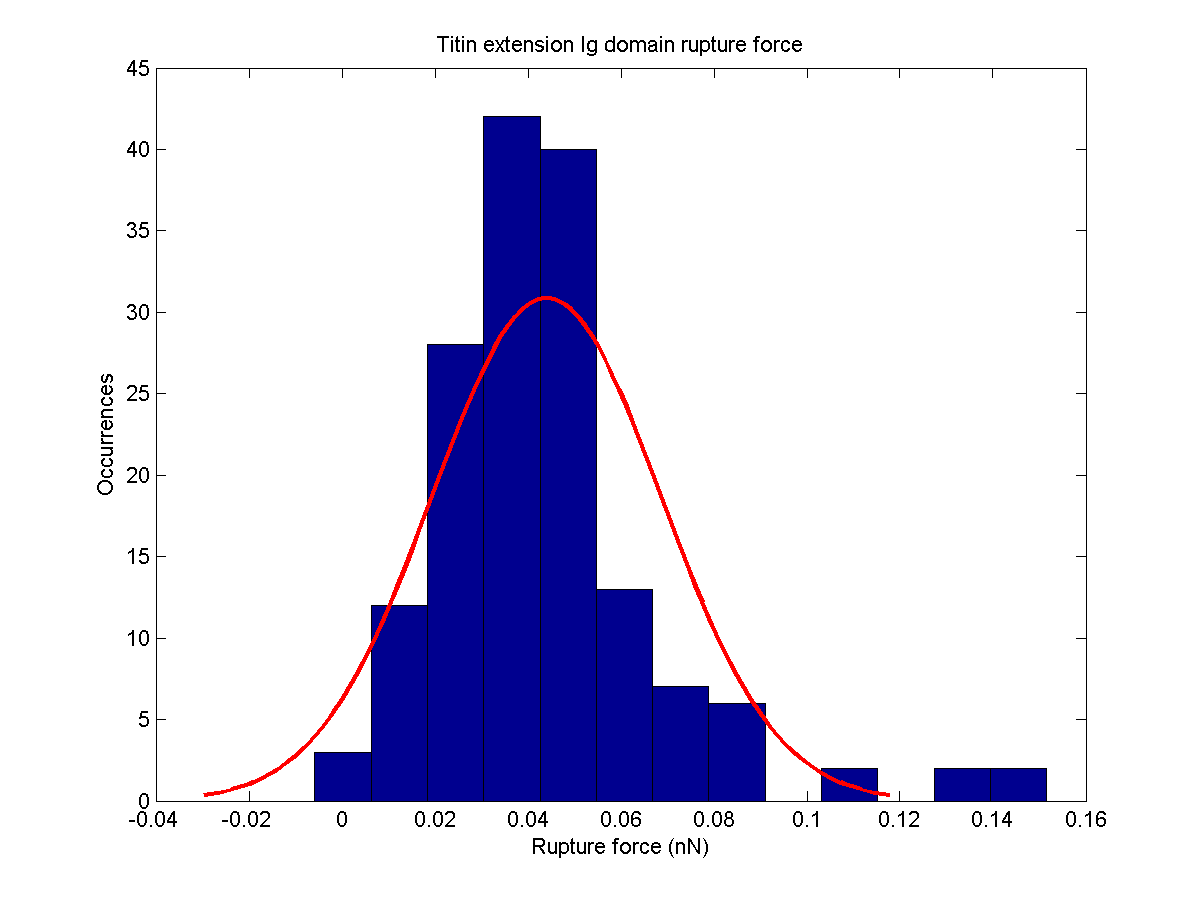
\includegraphics[width=0.8\textwidth]{hisrupt}
\centering
\caption{Ig domain zeroed rupture force fitted with a Gaussian distribution.}
\end{figure}

This value for the rupture force is subject to the same uncertainties as the contour length
not only in the values of the force peaks relative to each other, bu to the choice of zero.
The variability of the AFM calibration and the post-dissociation data means that even our 
most informed choice for zero is uncertain.

\subsection{Domain Contour and Persistence Length: Least Square
Curve Fitting of Force Peaks}

The worm-like chain model described in Equation (1) above suggests that a stretched
polymer applies zero resistance force in a completely folded state, and at its contour
length the force it applies diverges asymptotically. The forces binding a titin molecule to
the slide and the cantilever tip are small and finite, as are the hydrogen bonds and van
der Waals forces that fold titin. Therefore, the peaks seen in the AFM force-extension
curves, even if they did fit the WLC model, do not start at zero and do not stretch to the
contour length length. This claim would seem to discount the first to last average and
peak-to-peak values calculated above, but only insofar as we accept the WLC model.
Using least-square curve fitting functionality included in
MATLAB\footnote{MATLAB function \texttt{lsqcurvefit(fun,x0,xdata,ydata)} used in
scripts \texttt{zs\textunderscore wlcfit1.m} and \texttt{zs\textunderscore wlcfit5.m}.},
WLC model curves were fit to individual force-extension peaks. Fit curves plotted over
the force extension data are included in Figure 7. However, these fits were performed without
properly zeroing the extension scale. Thus, the average contour length from 14 peak fits
with the WLC model is 422 nm and the persistence length is 6.83 nm with standards of 
deviation 81 nm and 4.89 nm, respectively. These values are 
clearly  not consistent with those previous.

\begin{figure}[H]
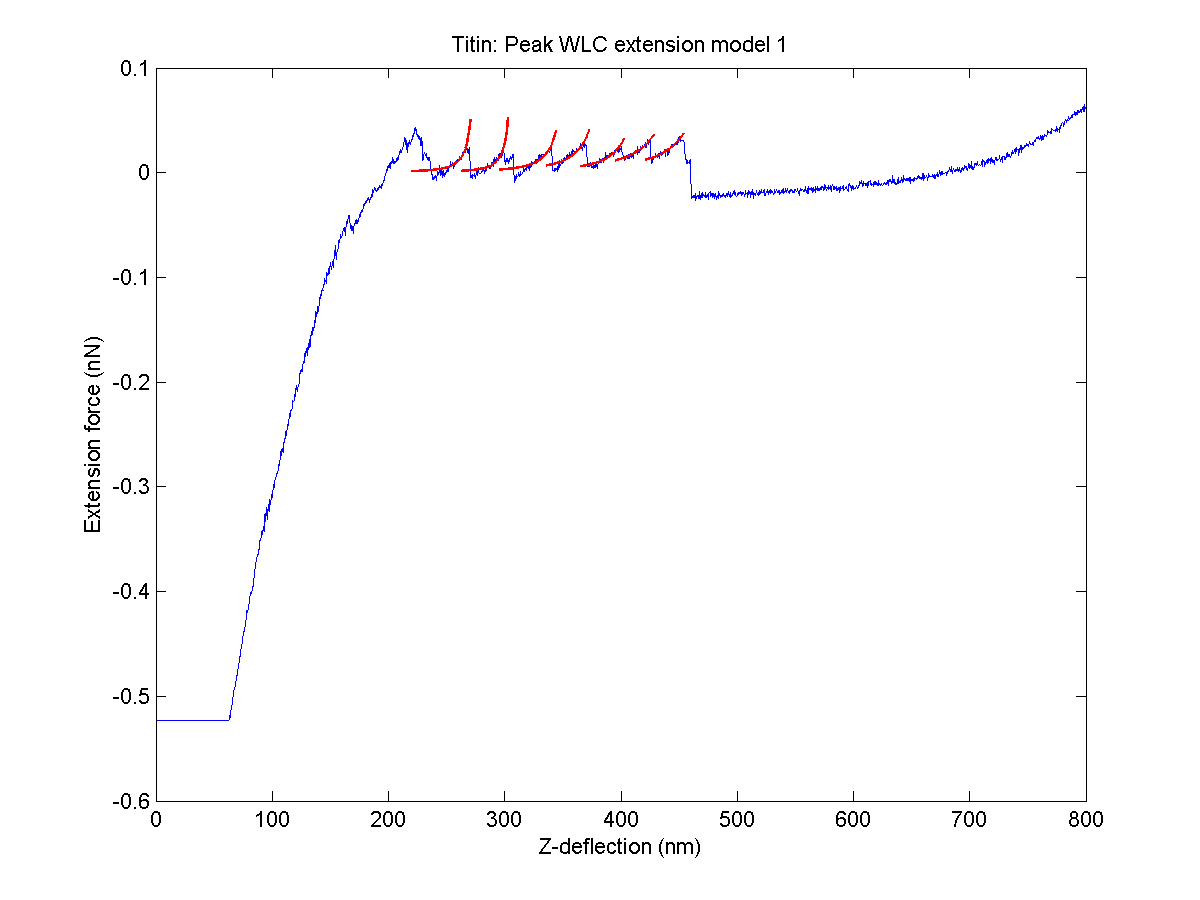
\includegraphics[width=0.8\textwidth]{wlc1_2-8}
\centering
\caption{Direct fitting of the worm-like chain model to titin force-extension data.}
\end{figure}

The results of an attempt\footnote{MATLAB script \texttt{zls\textunderscore wlcfit5.m}.}
to zero the extension scale for fitting with the WLC model 
is shown in Figure 8. Fiddling with initial guesses for the persistence and contour lengths
in the curve fitting procedure and arbitrary selecting the individual extension event zero 
point as the displacement two peaks before gave the best, but still not satisfactory, fit.
In fact, this procedure was only successful for one of the two force-extension curves
fitted without adjusting the zero. Also, though this method generates visually pleasing
plots, this choice of zero is otherwise unjustified. For 7 peaks fit with the WLC model, the
average contour length is 12.2 nm and the average persistence length is 0.62 nm with
standards of deviation 6.0 nm and 0.24 nm, respectively. This value for contour length
is now within two standards deviation of those calculated previously.

\begin{figure}[H]
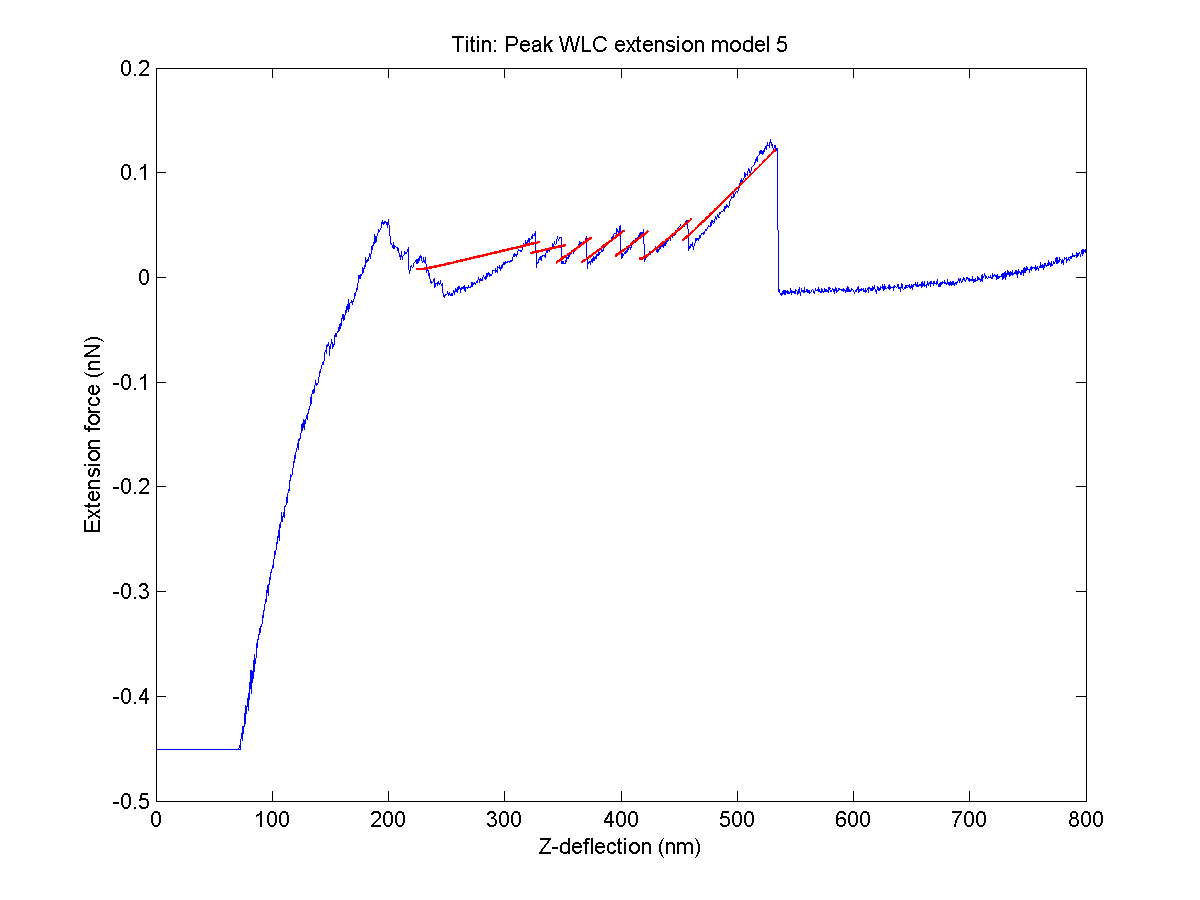
\includegraphics[width=0.8\textwidth]{wlcs5_3-9}
\centering
\caption{Worm-like chain model fitting of zero-adjusted titin force-extension data.}
\end{figure}

\section{Discussion}

Literature values for titin Ig27 domains give a non-fully extended peak spacing
of 25.4 nm \cite{biophysics} and approximately 28 nm \cite{nature}, unfolding force of
approximately 200 pN \cite{nature}\cite{biophysics}, and persistence
length 0.66 nm \cite{nature} and 0.29 nm \cite{biophysics}. Li et al. also includes a force of
29.2 pN as that at which the probability of unfolding  is 0.5.
The first to last over peaks separation, the peak to peak separation, and the zero-adjusted
WLC fitting value for $L_c$ are all within a standard of deviation of the reported peak to peak
spacing values. As discussed previously, these values likely correlate to the contour length
of the Ig domains, but likely is smaller than the true value.
The zero-adjusted WLC fitting value for the persistence length $P$ is just outside of a 
standard of deviation of the persistence length reported by \cite{biophysics}, but quite close
to that reported by \cite{nature}. The values from direct fitting are not even close.
The average of the zero-adjusted rupture forces calculated here is well below the literature 
value. However, this average is within a standard of deviation above the force for 50\%
probability of unfolding reported by \cite{nature}.
Along with the deviations from the procedure reported in Theory and Methods, I note
that the instruments used in the literature experiments were obviously far more precise
than those available for this laboratory exercise. The depth of exploration available
to those authors were greater and more complex than those we sought. For example,
their AFM probes were able to resolve a force transition within the first force-extension
peak which required theory beyond the WLC model in kinetics to explain.

The persistence length calculated from the zero-adjusted WLC model fit is about 20 times
the estimated length of an amino acid backbone and the calculated peak separation
is about 1000 times the length of an amino acid backbone. These ratios seem appropriate 
given the rigidity of the peptide bond, especialy under the influence of intramolecular forces
such as hydrogen bonding and van der Waals forces which contribute rigidity.

This lab elucidates the nature of protein mechanics, while emphasizing the statistical, 
combinatorial, and mechanical limitations of the single molecule measurements. The
specific analysis of titin has applications to physical organic chemistry and biology
in the contributions of protein structure and folding to strength limitations. Deeper
investigations by \cite{nature} even explored the physiological value of different parts
of natural titin in, for example, protection from undue muscle stress. Further analysis of the
available data with the freely-jointed chain (FLC) model could affrim our results, as could
more measurements. More precise instruments would make our analysis easier. Better
precision or a better understanding of the polymer mechanics should better justify
zero-adjustments, which would in turn improve the WLC or FLC analysis. 

\begin{thebibliography}{9}

\bibitem{biophysics}
Higgins, M. J.; Sader, J. E.; Jarvis, S. P. Frequency Modulation Atomic Force Microscopy 
Reveals Individual Intermediates Associated with each Unfolded I27 Titin Domain. 
\textit{Biophys. J.} [Online] \textbf{2006}, 90, 640–647.

\bibitem{nature}
Li, H.; Linke, W. A.; Oberhauser, A. F.; Carrion-Vazquez, M.;
Kerkvliet, J. G.; Lu, H.; Marszalek P. E.; Fernandez, J. M. Reverse engineering of the giant
muscle protien titin.  \textit{Nature} [Online] \textbf{2002}, 418, 998-1002.

\end{thebibliography}

\end{document}